\documentclass{article}
\usepackage{graphicx}
\usepackage{hyperref}
\usepackage{amsthm}
\usepackage{amsmath}
\usepackage{amssymb}
\usepackage{listings}

\lstset{basicstyle=\ttfamily}

\newtheorem{definition}{Definition}

\title{\huge{\textit{Foundations of \\ Artificial Intelligence}}}
\author{Fabio Vokrri}
\date{October 2024}

\begin{document}

\maketitle
\newpage
\tableofcontents

\newpage
\section{Introduction}
There isn't a single definition of Artificial Intelligence: some define intelligence in terms of fidelity to human performance, while others prefer a formal definition of intelligence called \textbf{rationality}. Some consider intelligence to be a property of reasoning and thought process, while others focus on intelligent behaviour.  

From these two characterizations (human v. rational/ thought v. behaviour) there are four possible combinations that cross several scientific disciplines.

\subsection{Acting Humanly - Turing Test Approach}
Alan Turing proposed the Turing test, a mental experiment to answer the question whether or not a computer can think. The test is passed if a human interrogator, after posing some written questions, cannot tell if the written responses came from a person or a computer.

To pass the test, the computer would need the following capabilities:
\begin{itemize}
    \item Natural language;
    \item Knowledge representation;
    \item Automated reasoning;
    \item Machine learning.
\end{itemize}

\subsection{Thinking Humanly - Cognitive Modeling Approach}
In order to say that a program thinks like a human, we must know how humans think. We can learn about human thoughts in three ways:
\begin{enumerate}
    \item Introspection: trying to capture our own thoughts;
    \item Psychological experiments: observing human behaviour;
    \item Brain imaging: observing the brain in action.
\end{enumerate}

Once we have a precise theory of the mind, it can be said that if a program's input-output behaviour matches a corresponding human behaviour, that is evidence that some of the program's mechanisms could also be present in a human.

\subsection{Thinking Rationally - "Laws of thought" Approach}
Aristotele was the first to attempt to codify "right thinking" with his syllogisms, providing a way to yield correct conclusions given the right premises. These laws were supposed to govern the operation of the mind. This field is called \textbf{logic} and requires the knowledge of the world that is certain,  a condition rarely met in reality. The theory of probability fills the gap, allowing rigorous reasoning with uncertain information.

\subsection{Acting Rationally - Rational Agent Approach}
An agent is something that autonomously acts, perceives the environment, persists over a prolonged period of time, adapts to the changes and pursues a goal. A rational agent is one that acts to achieve the best outcome.
This approach of AI has prevailed throughout the field's history because it's more general and amenable to scientific approach than others. AI has focused on the study of agents that do the right thing.

\newpage
\section{Intelligent Agents}
\subsection{Agents and Environments}
An agent, as already said, is anything that can be viewed as perceiving its environment through sensors and acting through actuators. The environment is a part of the universe whose state we are interested in when designing the agent, that is what the agent sees and what is effected by the agent's actions.

We use the term \textbf{percept} to refer to the content that the agent's sensors are perceiving. A \textbf{percept sequence} is the complete history of everything the agent has perceived.

An agent's action at any given time depends on its built-in knowledge and on the entire percept sequence observed to date, but not in anything it hasn't perceived. Mathematically speaking, it can be said that an agent's behaviour is described by the agent function, that maps any given percept sequence to an action the agent can perform.

\subsection{Good Behaviour and Rationality}
We said that a good agent, a rational one, does the right thing, but what is the right thing to do?

For an AI the right thing to do is described by the notion of \textbf{consequentialism}: we evaluate an agent's behaviour based on its consequences. When we introduce an agent to the environment, it produces a sequence of actions according to the percepts it receives. These actions cause the environment to go through a sequence of states and, if this sequence is desirable, then the agent has performed well. This notation of desirability us captured by a \textbf{performance measure}, which is initially prompted to the agent by its designer.

So, what is rational to any given time depends on four main thing:
\begin{enumerate}
    \item Performance measure, which defines the criteria for success;
    \item Agent's prior knowledge of the environment;
    \item Actions that the agent can perform;
    \item Agent's percept sequence up to date.
\end{enumerate}

\begin{definition}[Rational Agent]
For each possible percept sequence, a rational agent should select an action that is expected to maximize its performance measure, given the evidence provided by the percept sequence and whatever built-in knowledge the agent has.
\end{definition}

\subsection{Nature of Environments}
Before approaching the design of a rational agent, we must think about \textbf{task environments}, that are the problem that the agent is trying to solve. The nature of the task environments directly affects the appropriate design for the agent.  We can group the performance measure, the environment, the actuators and the sensors, all in the heading of the task environment.

The range of the tasks environments that might arise in AI is vast, but can be categorized as shown in the the next paragraphs.

\subsubsection{Fully v. Partially Observable}
If an agent's sensors give it access to the complete state of the environment at each point in time, then we say that the task environment is fully observable.
A task environment is effectively fully observable if the sensors detect all aspects that are relevant to the choice of action. 
Fully observable environments are convenient because the agent doesn't need to maintain any interval state to keep track of the world.
An environment could be partially observable because of noisy and inaccurate sensors or because part of the state are missing from the sensor data. If the agent has no sensors, the environment is unobservable.

\subsubsection{Single v. Multi}
Whether or not there are more than one agent operating in the task environment. But not all actors in an environment can be considered agents. A key factor to identify an agent is whether an entity behaviour is best described as maximizing a performance measure whose value depends on another agent's behaviour. 
If an entity us trying to maximize its performance measure by minimizing another agent's performance measure, then we can call the environment \textbf{competitive}, otherwise is called \textbf{cooperative}.

\subsubsection{Deterministic v. Non-deterministic}
If the next state of the environment is completely determined by the current state and the action executed by the agent (or agents), then we can sat that the environment is deterministic, otherwise is non-deterministic.
If the environment is partially observable, it could appear to be non-deterministic.

\textbf{N.B.}: We say that the model is \textbf{stochastic} if it explicitly deals with quantified probabilities and it is non-deterministic if the probabilities are listed, but not quantified.

\subsubsection{Episodic v. Sequential}
In an episodic task environment, the agent's experience is divided into atomic episodes, in which the agent receives a single percept and performs a single action. Furthermore, the next episode does not depend on the actions taken in previous episodes. In sequential environments, on the other hand, the current decision can effect future decisions.

\subsubsection{Static v. Dynamic}
If the environment can change while an agent is deliberating, the environment is said to be dynamic for that agent, otherwise is static. Static environments are easy to deal with because the agent needs not to keep looking at the world while deciding on an action to take. If the environment does not change with the passage of time, but the agent's performance score does, the environment is said to be \textbf{semi-dynamic}.

\subsubsection{Discrete v. Continuous}
This distinction applies to the state of the environment, to the way time is handled, and the percepts and actions of the agent.

\subsubsection{Known v. Unknown}
This distinction does not apply to the environment, but to the agent itself, more precisely to the agent's state of knowledge about the lows of physics of the environment. In a known environment, the outcome of any possible action is given, otherwise the agent must learn how it works in order to make good decisions.

\subsection{The Structure of Agents}
The job of an AI is to design an agent's program that produces rational behaviour. There are four categories of agent programs:
\begin{enumerate}
    \item Simple reflex agent;
    \item Model-based agent;
    \item Goal-based agent;
    \item Utility-based agent.
\end{enumerate}

Each of this types of agents combine some components in particular ways to generate actions.

\subsubsection{Simple Reflex Agents}
The simplest kind of agent is the Simple Reflex Agent, that select actions on the basis of the current percept, ignoring all the percept history. The actions taken by this kind of agent are given by some condition-action rules, which are simple \textit{if-then-else} statements that return a single action based on the current status of the environment.

\begin{figure}[h]
    \centering
    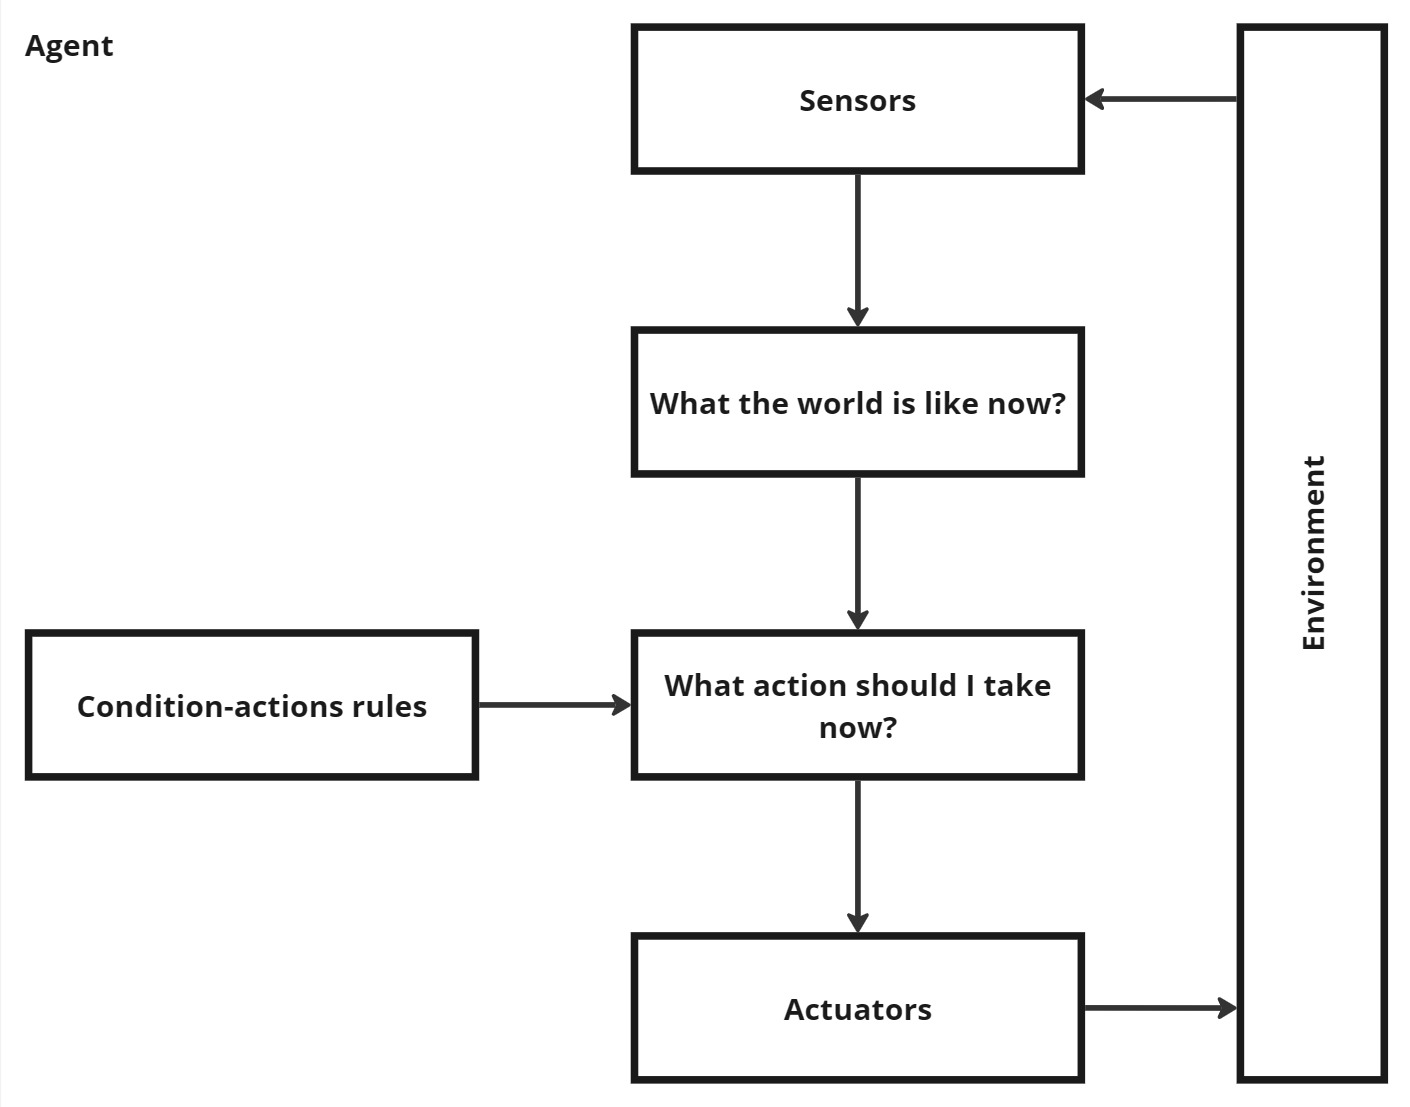
\includegraphics[width=0.75\linewidth]{images/Simple Reflex Agent.jpg}
    \caption{Simple Reflex Agent}
    \label{fig:simple_reflex_agent}
\end{figure}

Simple reflex agents are incredibly simple, but they are of limited intelligence. The agent will work only if the environment is fully observable and even a little bit of unobservability can cause the agent to fail.

Additionally, this kind of agents can fall into infinite loops of actions that are useless, given that have limited intelligence. To avoid this situation, some agents randomize actions, outperforming a deterministic version of the same agent. 

\subsubsection{Model-Based Reflex Agents}
The most effective way to handle partial observability is for the agent to keep track of the part of the world it cannot see at the moment. The agent should maintain some sort of internal state that depends on the percept history and therefore reflects some of the under-observed aspects of the environment.

\begin{figure}[h]
    \centering
    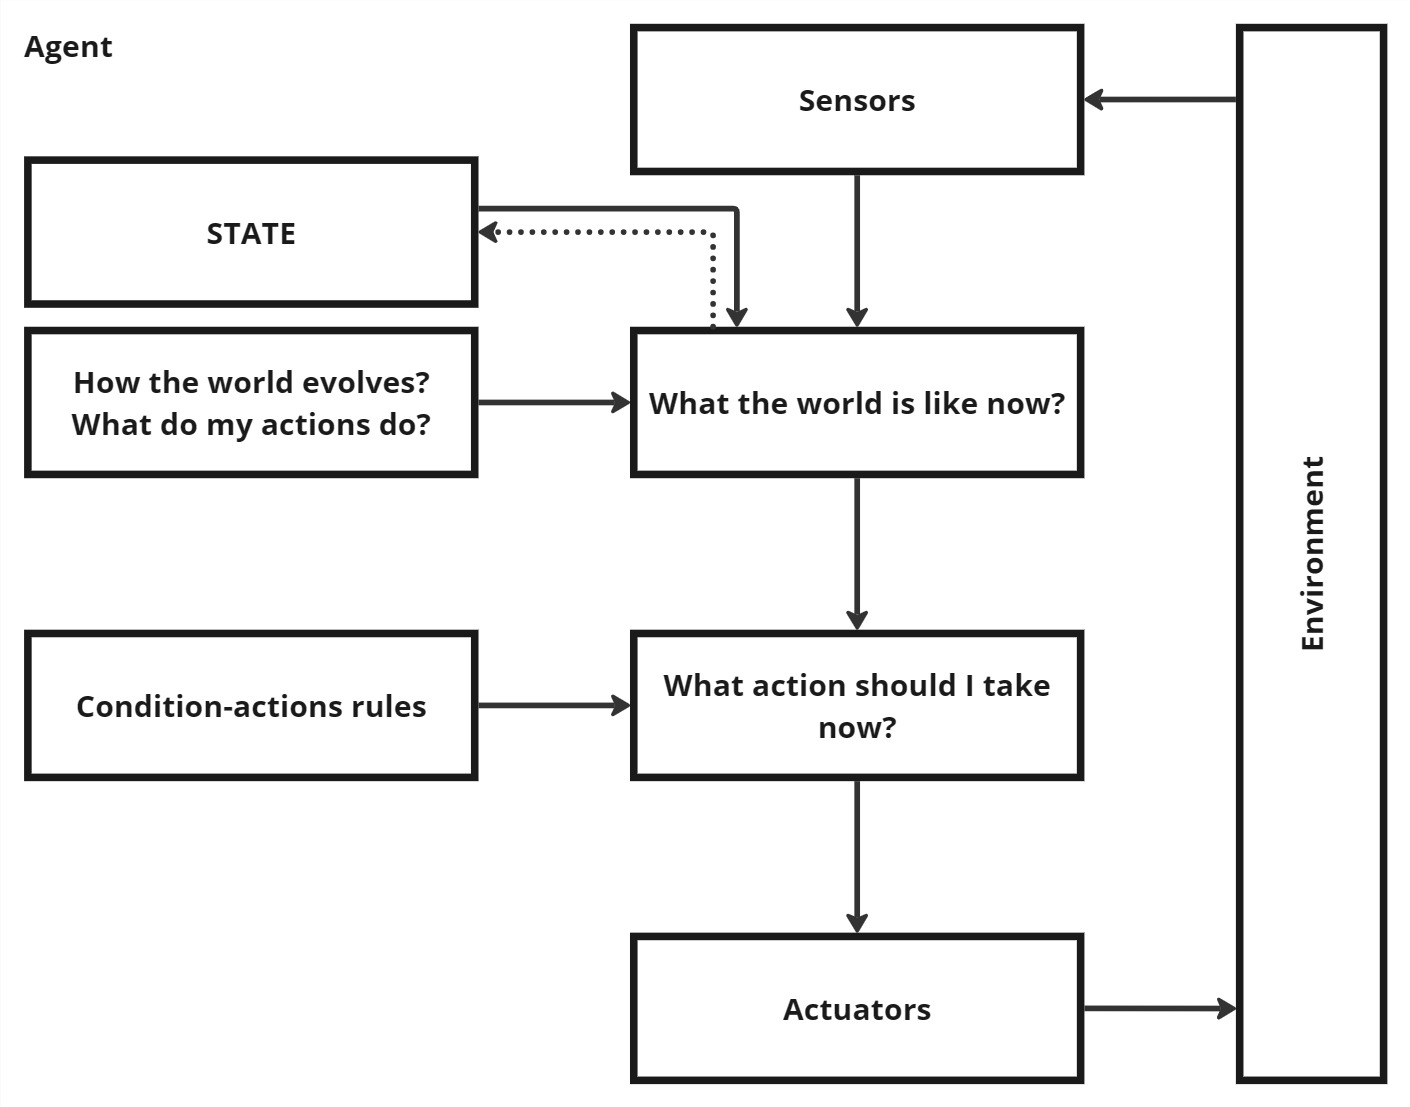
\includegraphics[width=0.75\linewidth]{images/Model Based Reflex Agent.jpg}
    \caption{Model Based Reflex Agent}
    \label{fig:model_based_reflex_agent}
\end{figure}

In order to update this internal state information, two kinds of knowledge are required to be encoded to the agent's program:

\begin{enumerate}
    \item Information about how the world changes over time, which can be divided in two parts:
    \begin{itemize}
        \item The effects of the agent's actions;
        \item How the world evolves independently of the agent.
    \end{itemize}
    This knowledge about how the world evolves is called a \textbf{transition model};
    \item Information about how the state of the world is reflected in the agent's percepts. This kind of knowledge is called \textbf{sensor model}.
\end{enumerate}

Together, the transition model and the sensor model allow the agent to keep track of the state of the world. An agent that uses such models is called a model-based agent.

\subsubsection{Goal-Based Agents}
Knowing something about the current state of the environment is not always enough to decide what to do. As well as the current state description, the agent needs some sort of \textbf{goal}, which are pieces of information that describe desirable situations.

The decision making part of this type of agent is different from the condition-action rules found in the model based reflex agents, in that involves some considerations of the future.

\begin{figure}[h]
    \centering
    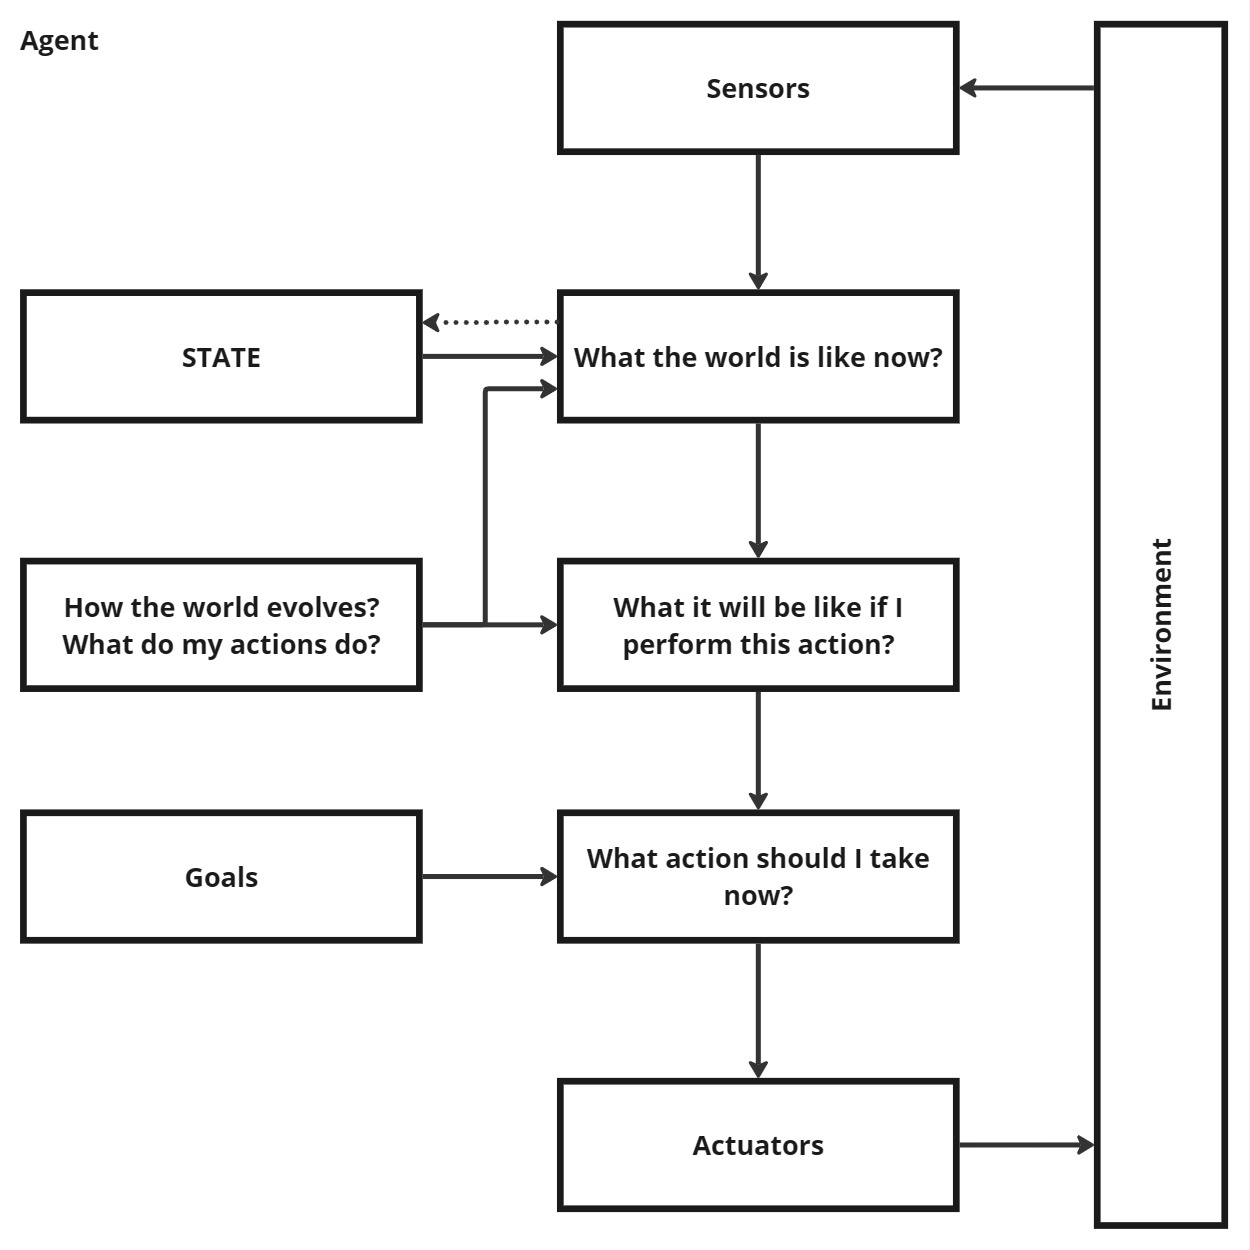
\includegraphics[width=0.75\linewidth]{images/Goal Based Agent.jpg}
    \caption{Goal Based Agent}
    \label{fig:goal_based_agent}
\end{figure}

Agents of this kind may appear less efficient than the ones analyzed up to now, but in reality they are more flexible because the knowledge that supports its decisions is represented explicitly and can be modified, simply by specifying the new goal.

\subsubsection{Utility-Based Agents}
Goals alone are not enough to produce high quality behaviour in most environments, because they only provide a crude distinction between \textit{"happy"} and \textit{"unhappy"} states. A more general performance measure should allow a comparison between different world states according to exactly how happy they would make the agent. In this field, a synonym of happy is \textbf{utility}.  

An agent's utility function is an internalization of the performance measure. Provided that the internal utility function and the external performance measure are in agreement, an agent that chooses actions to maximize its utility function will be rational according to the external performance measure. 

\begin{figure}[h]
    \centering
    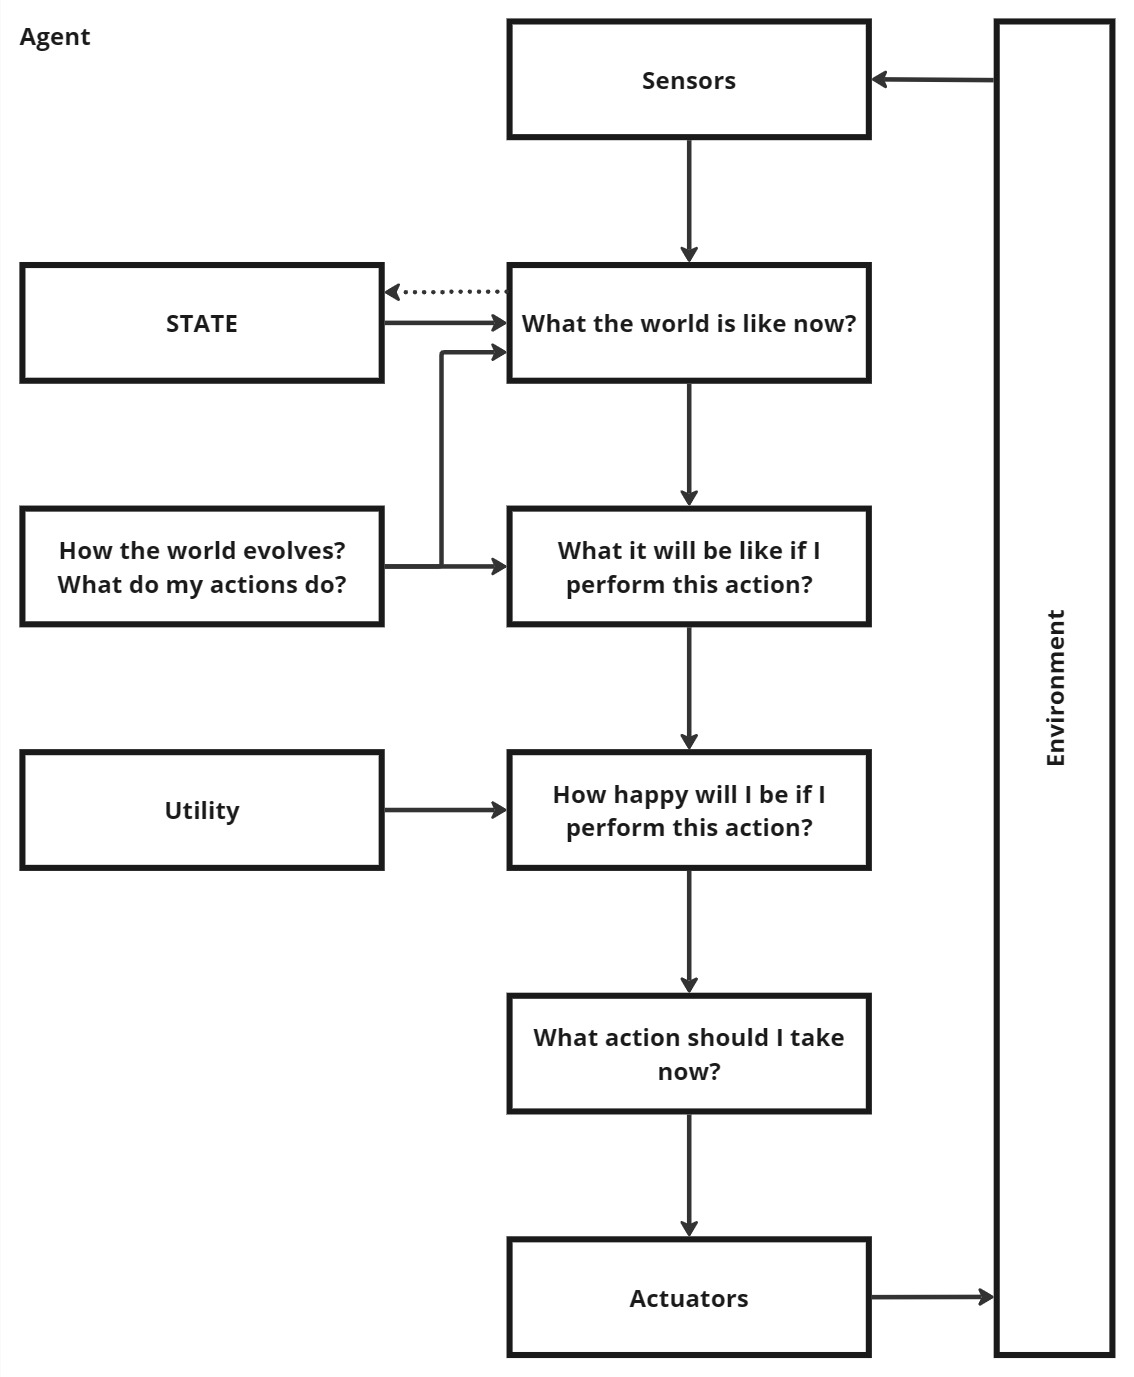
\includegraphics[width=0.75\linewidth]{images/Utility Based Agent.jpg}
    \caption{Utility Based Agent}
    \label{fig:utility_based_agent}
\end{figure}

There are two cases where goals are inadequate, but utility-based agents can still make rational decisions:
\begin{enumerate}
    \item Where there are conflicting goals but only some of them can be achieved: in this case the utility function specifies the right trade-off between the two goals.
    \item Where there are several goals that the agent can aim for, none of which can be achieved with certainty: in this case the utility function provides a way in which the likelihood of success can be weighted against the importance of the goal.
\end{enumerate}

\section{Learning Agents}
Any type of agent, such as model-based, goal-based or utility-based, can be built as a learning agent to improve their performance. Learning allows the agent to operate in a initially unknown environment and to become more competent than its initial knowledge alone might allow. 

\begin{figure}[h]
    \centering
    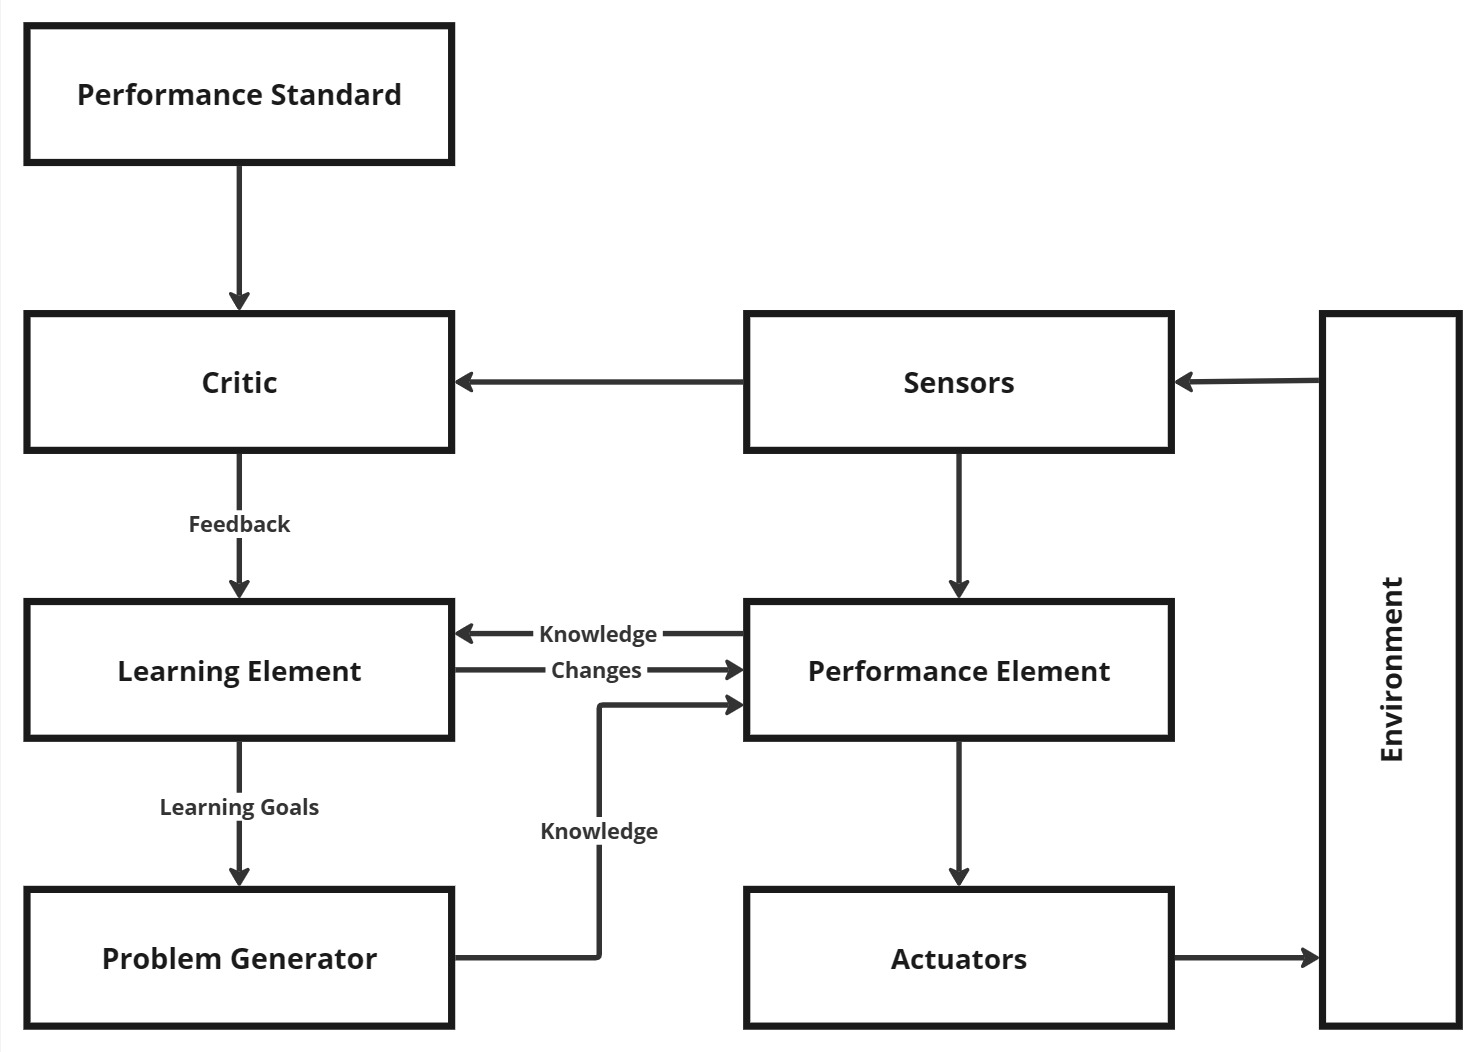
\includegraphics[width=0.75\linewidth]{images/Learning Agent.jpg}
    \caption{Learning Agent}
    \label{fig:learning_agent}
\end{figure}

It can be divided in four conceptual components:
\begin{enumerate}
    \item Learning element: responsible for making improvements;
    \item Performance element: analyzes the sensor input data and selects external actions. It's what we considered as the entire agent in the previous chapter;
    \item Critic: provides feedback on the actions taken by the agent and determines how the performance element should be modified to improve performance;
    \item Problem generator: suggests exploratory actions that lead to new and informative experiences. 
\end{enumerate}
\
\begin{definition}
    A computer program is said to learn from experience \textbf{E} with respect to some class of tasks \textbf{T} and performance measure \textbf{P}, if it improves with the given experience.
\end{definition}

Formally, Machine Learning is a field of AI focused on building algorithms capable of learning by extracting knowledge from experience. The goal is to build programs that can make informed decisions on new unseen data.

\begin{figure}[h]
    \centering
    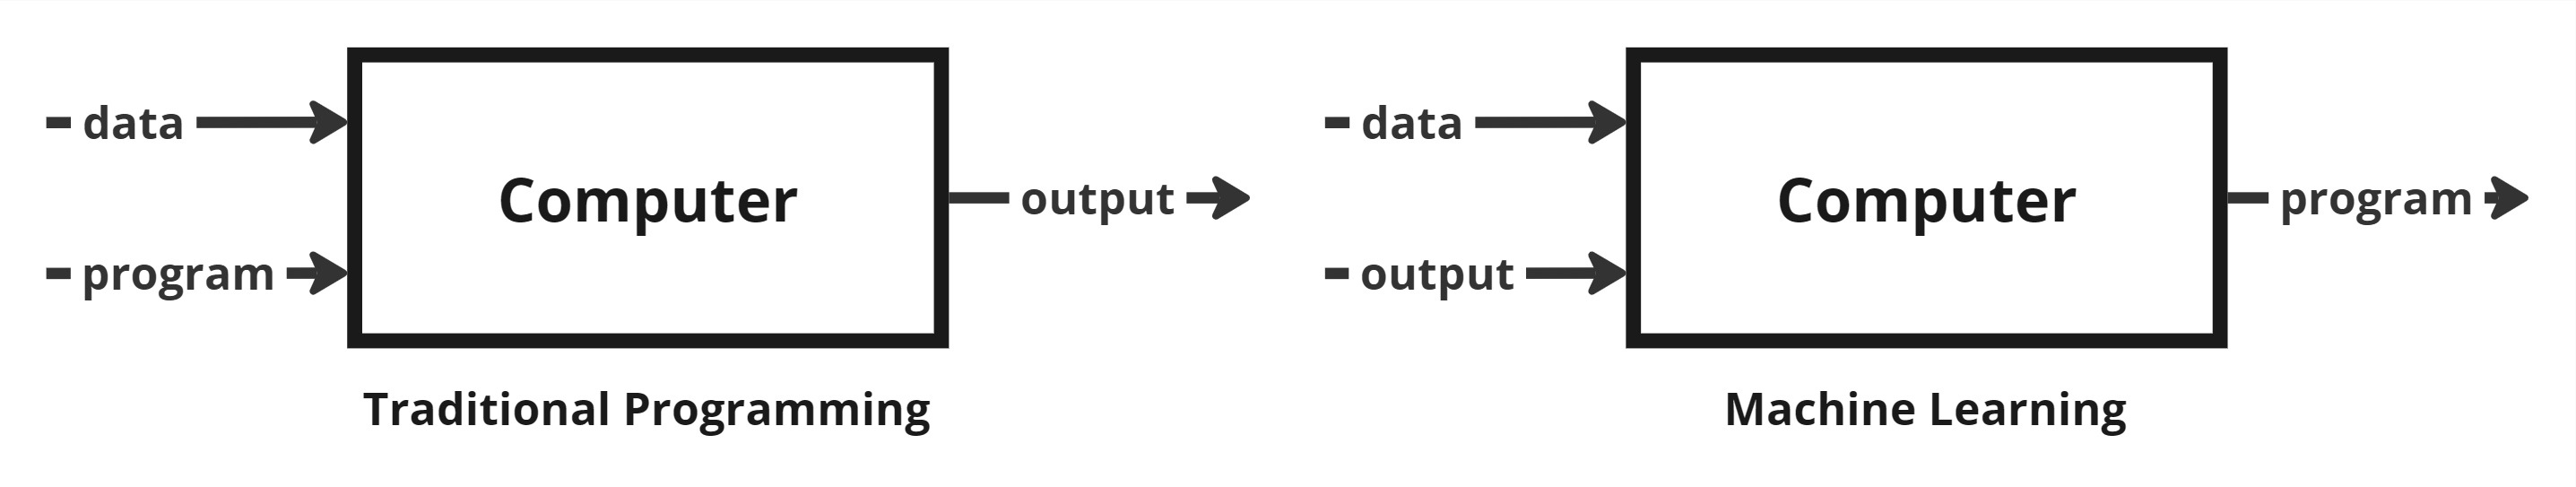
\includegraphics[width=0.75\linewidth]{images/Machine Learning Paradigm.jpg}
    \caption{Machine Learning Paradigm}
    \label{fig:machine_learning_paradigm}
\end{figure}

There are three main types of machine learning agents:
\begin{enumerate}
    \item \textbf{Supervised Learning}: given a set of desired outputs \(y_1, ..., y_n\), the agent learns to produce the correct output for a new set of unseen values. The outputs from which the agent learns are called \textbf{labels}.
    \item \textbf{Unsupervised Learning}: the agent exploits patterns and regularities in the experience collected (encoded as a dataset \(D = x_1, ..., x_n\)). In this case there's no desired output to predict and no feedback. The most common unsupervised learning task is called \textbf{clustering}, which detects useful clusters from the input example.
    \item \textbf{Reinforcement Learning}: the agent performs actions \(a_1, ..., a_n\) that effect the environment and receives a reward \(r\). The agent learns to maximize its long term reward. To do so, it needs:
    \begin{itemize}
        \item decision process;
        \item reward system;
        \item long term expectations;
        \item learning sequence of actions.
    \end{itemize}
\end{enumerate}

The most effective of these types of machine learning agents are the reinforcement learning ones, as they can learn from their own actions and experience, by considering their ultimate success or failure. In reinforcement learning, the agent perceives, at time \(t_0\), the environment to be in state \(s_{t_0}\) and decides to perform an action \(a_{t_0}\). As a result, in the next time step \(t_0+1\), the environment changes to state \(s_{t_0+1}\) and the agent receives a reward \(r_{t_0+1}\). 

The goal of the agent is to maximize the total amount of reward received by computing an action-value function that maps state-action pairs to expected payoffs:
\[Q(s_t, a_t) \to \textnormal{payoff}\]
or a state-value function mapping to expected payoffs:
\[V(s_t) \to \textnormal{payoff}\]

\subsection{Action Selection \& Policy}
At each time step, the agent must decide what action to take in step \(t=t_0\) based an its current evaluation of the expected payoff in \(s_t\) using a \textbf{policy function}. At any given point in time, the policy function \(\pi(s_t)\) selects what action the agent should perform based on its payoff evaluation.

When the correct action to take is not immediately obvious, an agent may need to consider a sequence of actions that lead to a goal state or, for short, to plan ahead of time. Such an agent is called \textbf{problem-solving agent} and the computational process is called \textbf{search}. The policy can be of two main types:
\begin{enumerate}
    \item deterministic: the policy function can be modeled as \(\pi: S \to A\). This type of policy can be conveniently represented as a table.
    \item stochastic: the policy function maps each state to a probability distribution over the actions. The function can be modeled as \(\pi: S\times A\to R\), which returns the probability of selecting the action \(a\) in state \(s\). Since \(\pi(s, a)\) is a probability distribution, it returns a value between 0 and 1, and the sum over all the actions is always 1.
\end{enumerate}

\
In order to obtain the maximum amount of reward, the agent must prefer actions that has tried in the past and found to lead to a high payoff. However, to discover those actions, it has to try actions that has never selected before. So the agent needs to find a trade-off between exploration of new actions and the exploitation of promising actions. This is called \textbf{exploration-exploitation dilemma}. 

Policies can be further divided into two categories:
\begin{enumerate}
    \item Greedy policies: for each state the policy deterministically selects an action with maximal value.
    \item \(\varepsilon\)-Greedy policies: with probability \(\varepsilon\) the policy selects a random action and with probability \(1-\varepsilon\) selects an action promising the highest payoff.
\end{enumerate}

\subsection{Environment}
The environment must satisfy the Markov property: the next state \(s_{t+1}\) and reward \(r_{t+1}\) only depend on the current state \(s_t\) and the taken action \(a_t\). Thus, the environment can be modeled as Markov Decision Process (MDP for short), which has a one-step dynamic described by the probability distribution \(p(s_{t+1}, r_{t+1}|s_t, a_t)\) such that:
\[p:S \times R \times S \times A \to [0, 1]\]
\[\sum_{s'\in S}\sum_{r\in R} p(s', r| s, a) = 1 \;\; \forall s \in S, \forall a \in A(s)\]

\subsection{Expected Payoff}
In reinforcement learning, the agent has to maximize the reward it receives in the long run, such that
\[G_t = r_{t+1} + r_{t+2} + ... + r_{t+k} + ... \to \infty\]
As shown, the problem with the \(G\) function is that it tends to add up to infinity. To provide an upper bound to the payoff, we introduce a discount factor \(\gamma\), such that \(0 < \gamma < 1\) for future rewards, obtaining the following function
\[G_t = r_{t+1} + \gamma \cdot r_{t+2} + \gamma^2 \cdot r_{t+3} + ... + \gamma^{k-1} r_{t+k} + ... < \infty \]

Thus, the expected reward to maximize would be defined as
\[\mathbb{E}[G_t] = \mathbb{E}\left[\sum_{k=0}^{\infty}\gamma^k r_{t+k+1}\right]\]

\subsection{Value Function}
The action-value function \(Q(s_t, a_t)\) estimates the expected future payoff when performing action \(a_t\) in state \(s_t\). The state-value function \(V(s_t)\) estimates the expected future payoff starting from state \(s_t\). Both functions can be decomposed as the sum of the immediate reward received \(r_{t+1}\) and the future rewards, so they become:
\[V(s) = \mathbb{E}[r_{t+1}+\gamma V(s_{t+1}|_{s_t=s})]\]
\[Q(s,a) = \mathbb{E}[r_{t+1}+\gamma  V(s_{t+1}|_{s_t =s, a_t = a})]\]

An agent based on the \(Q\) function is called a \textbf{Q-learning agent}. At the beginning, the table \(Q(\cdot, \cdot)\) is filled with random values, but at any time \(t\) the table is filled with the values provided by the following formula:
\[Q(s_t, a_t) = Q(s_t, a_t) + \beta(r_{t+1} + \gamma  \max_{a\in A}Q(s_{t+1}, a) - Q(s_t, a_t)) \]
where:
\begin{itemize}
    \item \(\gamma\) is the discount factor;
    \item \(\beta\) is the learning rate;
    \item \(\pi(s_t, a_t)\) is the action selection strategy: the \(\varepsilon\)-greedy policy is commonly used during learning, but sufficient exploration must guarantee to tackle the exploration-exploitation dilemma.
\end{itemize}

Tabular representation in q-learning agents is mostly infeasible in practice so approximators must be used. Reinforcement learning computes an unknown value function while also trying to approximate it. Approximators work on intermediate estimates while providing information for the learning agent. 

\newpage
\section{Solving Problems by Searching}
We will consider the simplest of environments only: episodic, single agent, fully observable, static, deterministic, discrete and known.

\subsection{Problem Solving Agents}
Any problem solving agent follows a process divided in four phases:
\begin{enumerate}
    \item \textbf{Goal formulation}: the agent adopts the goals. The goal is useful to organize behaviour by limiting the objectives and hence the actions to be considered.
    \item \textbf{Problem formulation}: the agent devises a description of the states and actions necessary to reach the goal. This description is an abstract model of the relevant parts of the world.
    \item \textbf{Search}: before taking any action, the agent simulates sequences of actions in its model, searching until it finds a sequence that reaches the goal. Such a sequence of actions is called a \textbf{solution}. The agent may simulate multiple sequences that do not reach the goal, but eventually it will find a solution, or it will find that no solution is possible.
    \item \textbf{Execution}: the agent executes the actions found in the solution sequence.
\end{enumerate}
\
A search problem can be defined as follows:
\begin{enumerate}
    \item A set of states in which the environment can be in, called the \textbf{state space};
    \item The initial state the agent starts in;
    \item A set of one or more goal states;
    \item The actions available to the agent. Given a state \textit{s}, the function \lstinline{ACTION(s)} return a finite set of actions the agent can perform in the given state. Such state are called \textbf{applicable} in \textit{s};
    \item A transition model, which describes what each action does. The function \lstinline{RESULT(s, a)} returns the state in which the agent will transition to performing action \textit{a} from state \textit{s};
    \item An action cost function, denoted by the \lstinline{ACTION-COST(s, a, s')} function, which returns the numeric cost of performing action \textit{a} in state \textit{s} to reach state \textit{s'}. A problem solving agent should use a cost function that reflects its own performance measure.
\end{enumerate}
\
A sequence of actions is called \textbf{path}. A solution is a path that leads form the initial state to a goal state. The total cost of a path is the sum of the individual costs of every action in the path. An optimal solution is the one that has the lowest path cost among all solutions.

The state space can be represented as a graph in which the vertices are the states and the directed edges between them are the actions the agent can perform. 

The formulation of the problem is the model, an abstract mathematical description. The process of removing irrelevant details from a representation is called \textbf{abstraction}. The abstraction is valid if we can elaborate any abstract solution into a solution in the more detailed world, and is useful if carrying out each of the actions in the solution is easier than the original problem. A good abstraction involves removing as much details as possible while retaining validity and ensuring that the abstract actions are easy to carry out.

\subsection{Search Algorithms}
A search algorithm takes a search problem as input and returns a solution. Most of these type of algorithms are based on a \textbf{search tree data structure} superimposed over the state graph, following various path from the initial state trying to find the one that reaches the goal state. Each node in the search tree corresponds to a state in the state space, while the edges of the tree correspond to actions, as seen in the state graph. The root of the tree corresponds to the initial state of the problem. 

The state space describes the possibly infinite set of states in the world and the actions that allow transitions from one state to another. The search tree describes paths between these states, reaching towards the goal. The search tree may have multiple paths to any given state, but each node has a unique path back to the root of the tree. 

The search tree is created by expanding every node considering the available actions for that state. To do so, we can use the \lstinline{RESULT} function to see where those actions lead to, and generating a new node for each of the resulting states. Now, the algorithm must choose which of these child nodes to consider in order to further expand the tree. This is the core of different search algorithms: they differ from each other for the way they choose the next child to expand in the tree. The set of states that haven't yet been expanded is called \textbf{frontier}, which separates the state space graph from into two regions:
\begin{itemize}
    \item The region of states that have been analyzed and, thus, expanded;
    \item The region of states that haven't yet been expanded.
\end{itemize}

\subsubsection{Best-First Search}
A general approach for deciding which node to expand from the frontier is the \lstinline{BEST-FIRST-SEARCH}, in which we choose a node \textit{n} with minimum value of some evaluation function \(f(n)\). On each iteration we choose a node of the frontier with the minimum value of \(f(n)\), return it if its state is the goal state, or call the \lstinline{EXPAND} function to generate its child nodes. Each child node is added to the frontier if it has not been reached before, or is re-added if it is reached by a path with a lower costing path. The algorithm returns either an indication of failure if a path is not found, or a node that represents a path to a goal. By using different \(f(n)\) functions, we obtain different search algorithms.

\subsubsection{Search Data Structures}
A node in the search tree is represented by a data structure that requires four components:
\begin{enumerate}
    \item \lstinline{node.STATE}: the state to which the node corresponds;
    \item \lstinline{node.PARENT}: the node in the tree that generated this node;
    \item \lstinline{node.ACTION}: the action applied to the parent node's state to generate this node;
    \item \lstinline{node.PATH-COST}: the total cost of the path from the initial state to this node.
\end{enumerate}

Following the \lstinline{PARENT} pointers back from a node, allows to recover the states and actions along the path to that node. Doing so from a goal node to the root of the tree we obtain the solution to the problem we are analyzing. 

Also a data structure to store the frontier is needed. Different data structures make up different types of searching algorithms. The main ones are:
\begin{itemize}
    \item Priority queue: pops the node with the minimum cost according to some evaluation function;
    \item Queue: pops the first node added to the queue;
    \item Stack: pops the last node added to the stack.
\end{itemize}

The reached states can be stored in a hash table, where each key is a state and each value is a node.

\subsubsection{Redundant Paths}
In the search tree might be repeated states, generated by a cycle (called a loopy path) in the graph over which the tree data structure was superimposed. So, there may be cases where the state space ha a finite amount of states, but the complete search tree is infinite, because there are no limits on how many times a path can be traversed in a loop. This kind of paths are called \textbf{redundant paths}, which represent an obstacle in solving the AI related problems. 

If we can eliminate redundant paths, we can make the searching algorithm order of magnitude faster. There are three main approaches to this issue:
\begin{enumerate}
    \item We can store all the previous traversed states in a separate data structure and detect redundant paths in order to keep only the best paths for each state. This approach is appropriate for state spaces where there are many redundant paths and the table of reached states fits in memory.
    \item We can not worry about repeating paths: in some problems is rare or even impossible for two paths to reach the same state, so we can save memory by not tracking reached states and redundant paths. We call a search algorithm a \textbf{graph search} if it checks for redundant paths and \textbf{tree-like search} if it does not.
    \item We can compromise and check only for cycles, but not for redundant paths in general. Since each node has a pointer to its parent node, we can check for cycles simply by following the chain of parents and verify if we land on the same state twice.
\end{enumerate}

\subsubsection{Performance}
An algorithm's performance can be evaluated in four main ways:
\begin{enumerate}
    \item Completeness: whether or not the algorithm is guaranteed to find a solution when there is one and to correctly report failure when there are no solutions;
    \item Cost optimally: whether or not the algorithm finds the most optimal solution, thus the path with the lowest cost of all solutions;
    \item Time and Space complexity: how long does the algorithm take to find a solution and how much memory does it need.
\end{enumerate}

To be complete, a search algorithm must also be \textbf{systematic} in the way it explores an infinite state space, making sure it can eventually reach a goal state which is connected to the initial state. In theoretical computer science, the complexity of a search algorithm is calculated based on the size of the state space graph, which is \(|V|+|E|\), where \(|V|\) is the number of vertices (or states) of the graph and \(|E|\) is the number of edges (or distinct state-action pairs). 

This calculation can be appropriate when the state graph is represented by an explicit data structure, but in AI related problems, this is not always the case. In fact, the graph is generally represented only implicitly by the initial state, actions and transition model. In this case, the complexity of a search algorithm can be measured in terms of the following parameters:
\begin{itemize}
    \item \textit{d} - depth: the number of actions in an optimal solution;
    \item \textit{m}: the maximum number of actions in any path;
    \item \textit{b} - branching factor: the number of successors of a node that need to be considered. 
\end{itemize}

When the branching factor is high, the number of nodes grows quickly and so does the problem complexity. When the depth is large, the closest solution requires more exploration of the search tree, making the algorithm slower. Sometimes, the depth is fixed for any solution.

\subsection{Uninformed Search Strategies}
In uninformed search algorithms no clue is given about how close a state is to the goal and only the information contained in the formulation of the problem itself is used.

\subsubsection{Breadth-First Search}
When all actions inside the state space have the same cost, an appropriate strategy would be a \textbf{breadth-first search}, in which the root node is expanded, then all its successors are expanded next, then their successors and so on. This algorithm is systematic and is therefore complete even on infinite states spaces.

We can implement this strategy by repeatedly calling the \lstinline{BEST-FIRST-SEARCH} algorithm where the evaluation function \(f(n)\) is the depth of the node. However, a more efficient implementation would be with a FIFO queue, giving us the correct order of nodes: new nodes (which are deeper than their parents) go to the back of the queue, and old nodes get expanded first, as they are shallower than the new nodes.

Breadth first search always finds a solution with the minimal number of actions, because when it is generating nodes at depth \textit{d}, it has already generated all the nodes at depth \textit{d}-1: if one of them were a solution, it would have been found and the algorithm would have terminated. This means that it is cost optimal for problems where all the actions have the same cost.

In order to calculate time and space complexity, we imagine that all nodes in the tree have \textit{b} successors. In this case, the root of the tree generates \textit{b} nodes, each of which generates \textit{b} more nodes, obtaining \(b^2\) nodes for the second level. Each of these generates \textit{b} more nodes, yielding \(b^3\) nodes at the third level and so on. All these generated nodes remain in memory, so both time and space complexity are \(O(b^d)\).

\subsubsection{Uniform-Cost Search}
When actions in the state space have different costs, an obvious choice would be to apply the \lstinline{BEST-FIRST-SEARCH} algorithm, where the evaluation function is the cost of the path from the root to the current node. This type of search is called \textbf{uniform cost search}. The idea behind this type of algorithm is to expand the nodes in waves of uniform path-cost, instead of uniform depth as in the breadth-first search.

The complexity of this algorithm is characterized in terms of \(C^*\), which is the cost of the optimal solution, and \(\varepsilon > 0\), which is a lower bound on the cost of each action. Then the algorithm's worst case time and space complexity is \(O(b^{1+\lfloor C^*/\varepsilon \rfloor})\), which can be much grater than the \(O(b^d)\) found for the breadth-first search algorithm. This is because uniform-cost search can explore very large trees of low-cost actions, before analyzing high-cost and perhaps useful actions.

\subsubsection{Depth-First Search}
This algorithm always expands the deepest node in the frontier list. The search proceeds immediately to the deepest level of the search tree, where the nodes have no successor. Then, if the goal state is not reached, it "backs up" to the next deepest node that still has unexpanded successors. 

It can be implemented using the \lstinline{BEST-FIRST-SEARCH} algorithm, where the evaluation function is the negative of the depth of the node. Alternatively can be implemented using a LIFO queue (also called stack) to represent the frontier: the generated successor nodes are inserted at the front of the frontier and the most recently generated nodes are selected first.

The depth-first search algorithm is not cost-optimal, as it returns the first solution it finds, even if it is not the cheapest one. For finite state spaces, it is efficient and complete, but in cyclic state spaces it can get stuck in an infinite loop. For this reason, some implementations of this algorithm check for loops for each new node in the frontier. Finally, for infinite spaces, it is not systematic either, because it can get stuck in infinite path that are not cycles.

Although it has some harsh downfalls, the depth-first search is generally used for its very limited memory usage: this algorithm has much smaller needs for memory, as it doesn't keep track of the reached states at all and it has a small frontier to save in memory. In fact, the depth-first search algorithm has a time complexity of only \(O(b\cdot m)\), where \textit{b} is the branching factor and \textit{m} is the maximum depth of the tree.

\subsubsection{Depth-Limited Search \& Iterative Deepening Search}
We can prevent the depth-first search algorithm to go on endless paths by limiting the depth at which the algorithm can go. We call this algorithm \textbf{depth-limited search}, with limit \(\ell\): we treat all nodes at that depth as if they had no successor. The time complexity of this algorithm is \(O(b^\ell)\) and the space complexity is \(O(b\cdot \ell)\). Unfortunately, if we choose an inappropriate value of \(\ell\), the algorithm will fail to reach a solution and it becomes incomplete again. Sometimes a good depth limit can be chosen based on the problem we are trying to solve, but for most problems we will not know a good depth value until we solve the problem.

\textbf{Iterative deepening search} solves the problem of finding a good value for \(\ell\) by trying all values until a solution is found or no solutions were found. This approach combines benefits from the depth-first search and breadth-first search algorithms. In fact, like depth-first search, the memory required is modest, spanning from \(O(b\cdot d)\) when there is a solution, to \(O(b\cdot m)\) on finite state spaces with no solutions. Like breadth-first search, iterative deepening search is optimal for problems where all the actions have the same cost, and is complete on finite acyclic state spaces, or on any finite state space when we check nodes for cycles all the way up the path. The time complexity is \(O(b^d)\) when there is a solution, or \(O(b^m)\) when there is none.

\subsubsection{Bidirectional Search}
One last strategy we can apply for uninformed search can be to go backward, from the solution to the initial state if the problem is easily reversible. A more efficient way is to combine the two directions into a bidirectional search: this type of search performs two searches in parallel, one \textit{forward} search from the initial state to the goal state, one \textit{backwards} search from a goal state to the initial state.

\subsubsection{Summary}

\begin{table}[h]
    \begin{tabular}{lcccc}
        \multicolumn{1}{l}{} & \multicolumn{2}{c}{\textit{With repeated states}} & \multicolumn{2}{c}{\textit{Without repeated states}} \\
        \multicolumn{1}{r||}{Search Strategy} & \multicolumn{1}{c|}{Complete} & \multicolumn{1}{c|}{Optimal} & \multicolumn{1}{c|}{Complete} & Optimal \\ \hline \hline
        \multicolumn{1}{l||}{\textbf{Breadth-First Search}} & \multicolumn{1}{c|}{YES} & \multicolumn{1}{c|}{YES} & \multicolumn{1}{c|}{YES} & YES \\ \hline
        \multicolumn{1}{l||}{\textbf{Uniform-Cost Search}} & \multicolumn{1}{c|}{YES} & \multicolumn{1}{c|}{YES} & \multicolumn{1}{c|}{YES} & YES \\ \hline
        \multicolumn{1}{l||}{\textbf{Depth-First Search}} & \multicolumn{1}{c|}{NO} & \multicolumn{1}{c|}{NO} & \multicolumn{1}{c|}{YES} & NO \\ \hline
        \multicolumn{1}{l||}{\textbf{Limited-Depth Search}} & \multicolumn{1}{c|}{NO} & \multicolumn{1}{c|}{NO} & \multicolumn{1}{c|}{NO} & NO \\ \hline
        \multicolumn{1}{l||}{\textbf{Iterative Deepening}} & \multicolumn{1}{c|}{YES} & \multicolumn{1}{c|}{YES} & \multicolumn{1}{c|}{YES} & YES
    \end{tabular}
    \caption{Strategy comparison}
    \label{tab:strategy_comparison}
\end{table}

\begin{table}[h]
    \centering
    \begin{tabular}{l||c|c}
        Strategy & S(n) & T(n) \\ \hline \hline
        \textbf{Breadth-First Search} & \(O(b^d)\)  & \(O(b^{d+1})\) \\ \hline
        \textbf{Uniform-Cost Search} & \(O(b^{1+\lfloor C^*/\varepsilon \rfloor})\) & \(O(b^{1+\lfloor C^*/\varepsilon \rfloor})\) \\ \hline
        \textbf{Depth-First Search} & \(O(bm)\) & \(O(b^m)\) \\ \hline
        \textbf{Limited-Depth Search} & \(O(b\ell)\) & \(O(b^\ell)\) \\ \hline
        \textbf{Iterative Deepening} & \(O(bd)\) & \(O(b^d)\) \\
    \end{tabular}
    \caption{Strategy Complexity}
    \label{tab:strategy_complexity}
\end{table}

Where:
\begin{itemize}
    \item \(b\) is the number of successors of a node that need to be considered;
    \item \(d\) is the number of actions in an optimal solution;
    \item \(m\) is the maximum number of actions in any path;
    \item \(C^*\) is the cost of the optimal solution;
    \item \(\varepsilon\) is the lower bound on the cost of each action;
    \item \(\ell\) is the depth limit;
\end{itemize}

\subsection{Informed Search Strategies}
In informed search algorithms, specific knowledge that is not contained in the problem formulation is exploited to solve the problem itself. This strategy selects a node from the frontier according to an evaluation function \(f(n)\), which provides an estimate of how much a node is "promising". There are two main ways to calculate the evaluation function:
\begin{enumerate}
    \item Greedy best-first search;
    \item A* search.
\end{enumerate}

Conventionally, the most promising nodes have a small value of the evaluation function \(f(n)\), so the frontier is implemented as a priority queue ordered in increasing order of \(f(n)\). Thus, nodes with the minimum \(f(n)\) are chosen first.

\subsubsection{Greedy Best-First Search}
Greedy best-first search algorithms use an evaluation function that is equal to the \textbf{heuristic function} \(h(n)\), which gives the \textit{estimated} cost of the cheapest path from the state at node \(n\) to a goal state. To apply the greedy best-first search, the function \(h(n)\) must be known. Note that, the heuristic is an estimate, not an actual cost: if we knew the actual cost of the path, the problem would have already been solved.

There are many heuristic functions we can choose for every given problem, but there are some more accurate than others. In fact, given two heuristic functions \(h_1(n)\) and \(h_2(n)\), such that \(h_1(n)\le h_2(n)\) for any node \(n\), \(h_2\) is said to dominate \(h_1\) since each node expanded using \(h_2\) is also expanded using \(h_1\). In this case we say that the function \(h_2\) is more accurate, or more informed, than the function \(h_1\).

Greedy best-first search is neither complete nor optimal, as it can get stuck in an infinite loop. The time and space complexity of this algorithm in the worst-case scenario are both \(O(b^m)\), where \(m\) is the maximum depth of the search tree (which could be infinite).

\subsubsection{A* Search}
The most used informed search algorithm is \textbf{A* search}, a best-first search that uses the evaluation function \(f(n) = g(n) + h(n)\), where:
\begin{itemize}
    \item \(g(n)\) is the path cost from the initial state to node \(n\) (what we know for sure);
    \item \(h(n)\) is the estimate cost of the shortest path from \(n\) to a goal state (what we are estimating).
\end{itemize}
Put in simpler words, \(f(n)\) is the estimated cost of the best path that continue from the state \(n\) to a goal state. By using both the cost so far and the estimated cost of reaching the goal, A* can lead the agent away from suboptimal paths.

A* search is complete and optimal for tree-search when the function \(h(n)\) is \textbf{admissible}. A heuristic function is admissible when, for each node \(n\), it is true that 
    \[0 \le h(n) \le h^*(n)\]
where \(h^*(n)\) represents the actual cost from the given node to a solution node. When \(n\) is a goal state, \(h(n)\) should be zero. An admissible heuristic is \textit{"optimistic"} since it always underestimates the true cost to reach the goal. In fact an it can be seen as the cost of an optimal solution to a relaxed problem, obtained by removing the constraints.

A* search is also complete and optimal for graph-search when the function \(h(n)\) is \textbf{consistent}. An heuristic function is consistent when, for every node \(n\) and every successor \(n'\) generated from \(n\) by action \(a\), it is true that 
\[h(n)\le c(n,a,n') + h(n') \;\; \textnormal{(triangular inequality)}\]
When \(n\) is a goal state, \(h(n)\) should be zero. Every consistent heuristic function is also an admissible one, but not vice versa. Consistency is a stronger property than admissibility, because graph-search is more constrained since it does not consider nodes corresponding to the same state, thus it requires a stronger property to guarantee completeness and optimality. In addition, with a consistent heuristic, the first time we reach a state it will be on an optimal path, so we never have to re-add a state to the frontier and never have to change an entry in the \textit{reached} set.

There are many types of consistent heuristic functions, but some of them are uninteresting: for example, the heuristic function \(h_0(n) = 0 \;\; \forall n\) is consistent and admissible, but it implements a uniform-cost search (uninformed search algorithm), so it is not really that interesting.

A special variation of the A* search is the \textbf{weighted A* algorithm}. It introduces a weight factor \(w\), which is \(1 \le w < \infty\), over the heuristic functions so that \(f(n) = g(n) + w \cdot h(n)\). The theoretical properties of the simple A* search do not apply anymore, but this extension of the algorithm can be more efficient and solve search problems quicker.

The last, and most successful, variation of A* search is the \textbf{iterative-deepening A* search} (IDA* search), which reduces memory requirements by applying a limit to the values of the evaluation function \(f(n)\). It is to A* what iterative-deepening was to depth-first search: IDA* gives all the benefits of A* without the requirement to keep the reached states in memory, at the cost of visiting some states multiple times. In IDA* the cutoff value is the \(f-cost (g+h)\); at each iteration, the cutoff value is the smallest \(f-cost\) of any node that exceeded the cutoff on the previous iteration. IDA* search is complete and optimal when the heuristic function \(h(n)\) is admissible.

\newpage
\section{Constraint Satisfaction Problems}
In standard search, the basic idea is that problems can be solved by searching the state space, that is a graph in which nodes represent states and edges between them represent actions. In this type of search algorithms, the states are atomic, indivisible, like a \textit{black box}: for each problem, we need domain-specific heuristic function to describe the transition between states.

In \textbf{constraint satisfaction problems}, \textbf{CSP} for short, we break open this black box by using a factored representation for each state, that consists of a set of variables, each of which have a value. A CSP is solved if each variable has a value that satisfies all the constraints on that variable.

CSP search algorithms take advantage of the structure of states and use a general heuristic to enable the solution of complex problems. The main idea is that we can eliminate large portions of the search space by identifying values that violate constraints on variables.  \\

\begin{definition}
A CSP consists of three components:
\begin{itemize}
    \item \(\mathcal{X} =\{X_1, ..., X_n\}\) is a set of variables;
    \item \(\mathcal{D} =\{D_1, ..., D_n\}\) is a set of domains, one for each variable;
    \item \(\mathcal{C}\) is a set of constraints that specify valid combinations of values.
\end{itemize}
\end{definition}

A domain \(D_i\) is a set of allowable values \(\{v_1, ..., v_k\}\) for each variable \(X_i\). Each constraint \(\mathcal{C}_j\) consists of a pair \(<scope,\; rel>\), where \(scope\) is a tuple of variables that participate in the constraint, and \(rel\) is a relation that defines the valid values for those variables. A relation can be represented as am explicit set of all tuples of values that satisfy the constraint, or as a function that can compute whether or not a tuple is a member of the solution.

The goal of the CSP is to assign values to the variables, such that 
\[\{X_i=v_i, X_j=v_j, ...\}.\] 
An assignment is \textbf{consistent} if does not violate any constraints and is \textbf{complete} if all variables are assigned a value. A solution to a CSP is a consistent and complete assignment. If all the domains have fixed size \(d\), there are \(O(d^n)\) complete assignments possible.

Every CSP can be visualized as a constraint graph: the nodes of the graph correspond to variables of the problem and the edge connects any two variables that participate in a constraint. This type of representation for the problem can dramatically speed up the search problem. Additionally, we will consider only binary constraints, in which only two variables are involved, because higher order constraints can be transformed in a CSP with only binary constraints through simple transformations.

\subsection{Constraints Propagation - Arc consistency}
A variable in a CSP problem is arc-consistent if every value in its domain satisfies the variable's binary constraints. More formally, \(X_i\) is arc-consistent with respect to another variable \(X_j\) if there is some value in the domain \(D_j\) that satisfies the binary constraint in the arch \((X_i, X_j)\).

The most popular algorithm for enforcing the arc-consistency property on a CSP problem is called \textbf{AC-3}, which maintains a queue of arcs to consider. Initially, the queue contains all the arcs in the CSP. Then, the algorithm pops off an arbitrary arc \((X_i, X_j)\) and makes \(X_i\) arc-consistent with respect to \(X_j\). If this leaves \(D_i\) unchanged, the algorithm moves on the next arc, but if this operation revises the domain \(D_i\) (making it smaller), then we add to the queue all arcs \(X_k, X_i\), where \(X_k\) is a neighbor of \(X_i\). This is necessary because, by reducing \(D_i\), we might enable further reductions in \(D_k\), even if we've already applied the algorithm to that node. If \(D_i\) is revised down to nothing, then we know that the whole CSP problem has no consistent solution and the algorithm can immediately return failure. Otherwise, we keep checking, trying to remove values from the domains of variables until no more arcs are in the queue. At this point we are left with a CSP equivalent to the initial one, but the arc consistent one will be faster to search because its variables have smaller domains.

The complexity of AC-3 is \(O(cd^3)\) in the worst case scenario.

\subsection{Backtracking Search for CSP}
Sometimes we can finish the constraint propagation process and still have variables with multiple possible values. In this case we have to search a solution. For a CSP problem with \(n\) variables of domain size \(d\) we would end up with a search tree where all the complete assignments are leaf nodes at depth \(n\). But, the branching factor at the top level would be \(nd\) because any of \(d\) values can be assigned to any of \(n\) variables. At the next level, the branching factor is \((n-1)d\) and so on for \(n\) levels. So the tree has \(n!d^n\) leaves, even though there are only \(d^n\) possible assignments.

We can remove the \(n!\) factor by recognizing that CSP have the \textbf{commutative property}. A problem is said to be commutative if the order of any given set of actions does not matter. In CSPs it makes no difference if we first assign a value to a variable first and then to another, or the other way around. Therefore, we need only consider a single variable at each node in the search tree. At each level of the tree we must choose which variable we will deal with, but we never have to backtrack over that choice. 

Backtracking search algorithm for CSP repeatedly chooses an unassigned variable and tries all values in the domain of that variable in turn, trying to extend each one into a solution recursively. If the call succeeds, the solution is returned, otherwise the assignment is restored to the previous state, from which we try all the remaining values. If no value works we return a failure. This algorithm can be improved by using domain-independent heuristics that take advantage of the factored representation of the CSP.

\subsubsection{Variable ordering}
There are various strategies we can implement in order to select an unassigned variable. The simplest one is to choose variables in order \(\{X_1, X_2, ..., X_n\}\) or randomly. Though, there are better heuristics, like choosing the variable with the fewest possible values, called \textbf{minimum-remaining-values} (\textbf{MRV}). This strategy is also called "fail-first" as it picks a variable that is most likely to cause a failure soon, thereby pruning the tree.

Another strategy is the \textbf{degree heuristic}, which attempts to reduce the branching factor on future choices by selecting the variable that is involved in the largest number of constraints on other unassigned variables. The MRV heuristic is usually more powerful, but the degree heuristic can be useful as a tie-breaker.

Once a variable is selected, the algorithm must decide on the order ti examine its values. An efficient algorithm is the \textbf{least-constraining-value} heuristic, which prefers the value that rules out the fewest choices for the neighboring variables in the constraint graph.

We learned that variables should be selected following the "fail-first" principle, while its values should follow the "fail-last" principle. This is because every variable has to be assigned eventually, so by choosing the ones that are likely to fail first, we will have fewer successful assignments to backtrack over. On the other hand, for value ordering we need only one solution, so it makes sense to look for the most likely values first.

\subsubsection{Forward Checking}
The AC-3 algorithm can reduce the domains of variables before we begin the search, but inference can be more powerful during the search. One simple type of inference is \textbf{forward checking}. Whenever a variable \(X\) is assigned, the forward checking algorithm establishes arc consistency for it: for each unassigned variable \(Y\) connected to \(X\) by a constraint, it deletes from \(Y\)'s domain any value that is consistent with the value chosen for \(X\). For many applications, the search is more effective if we combine the MRV algorithm with forward checking. A problem with forward checking is that although it detects many inconsistencies, it does not detect them all.

\subsection{Local Search}
We can efficiently solve CSPs using another paradigm: \textbf{local search}. It uses a complete state formulation where each state assigns a value to every variable, and the search changes the value of one variable at a time. To do so, it uses the \textbf{hill-climbing} algorithm: considering the states of a problem as laid out in a state-space landscape, each point has an "elevation", defined by the value of the objective function; the problems is narrowed down to finding the global maximum value. The only problem in this kind of algorithms is that they can stop at local maxima, yielding a sub-optimal solution.

\newpage
\section{Adversarial Search and Games}
Adversarial search problems are a set of problems in which we explore competitive environments, where two or more agents have conflicting goals.

\subsection{Two-Player Zero-Sum Games}
The most studied problems in AI are the deterministic, two-player, turn-taking, perfect information (fully observable) and zero-sum (there's always one winning player) games. In game theory the terms move and position are used as synonim for action and state respectively.

The analyzed games will always have two involved players, called MAX and MIN, in which MAX moves first and then the players take turns moving until the game is over. 

A game can formally be defined with the following elements:
\begin{itemize}
    \item \(S_0\): the initial state, which specifies how the game is set up at the start;
    \item \lstinline{To-Move(s)}: the player whose turn it is to move in state \(s\);
    \item \lstinline{Actions(s)}: the set of legal moves the player can do in state \(s\);
    \item \lstinline{Result(s, a)}: the transition model, which defines the state resulting from the taking action \(a\) in state \(s\);
    \item \lstinline{Is-Terminal(s)}: the terminal test, which returns true if the game is in a terminal state, false otherwise;
    \item \lstinline{Utility(s, p)}: the utility function, which defines the final numeric value to player \(p\) when the game ends in terminal state \(s\).    
\end{itemize}

The initial state, the \lstinline{Actions} function and the \lstinline{Result} one define the \textbf{state space graph}, where the vertices represent the states and the edges the moves. As always a \textbf{search tree} can be superimposed on the graph (or on a particular part of it), to determine what moves to make next. We can define the complete \textbf{game tree} as the search tree that follows every possible path all the way down to a terminal state.
Leaf nodes contain the utility value of the terminal state from the point of view of MAX: high values are good for MAX and bad from MIN.

\subsection{Optimal Decisions}
Given a game tree, the optimal strategy can be determined by evaluating the \textbf{minimax} value of each state of the tree, which is indicated with \lstinline{MINIMAX(s)}. This value is the utility for MAX being in that state, \textit{assuming that both players play optimally}. The minimax value of a terminal state is just its utility. In any terminal space, MAX prefers to move to a state of maximum value when it's his turn to move, while MIN prefers a state of minimum, which is minimum value for MAX (thus maximum value for MIN). So the minimax function is calculated as follows:
\begin{multline}
    MINIMAX(s) = \\
    \begin{cases}
        Utility(s, MAX) & if \;\; Is-Terminal(s) \\
        \max_{a\in Actions(s)} MINIMAX(Result(s, a)) & if \;\; To-Move(s) = MAX \\
        \min_{a \in Actions(s)} MINIMAX(Result(s, a)) & if \;\; To-Move(s) = MIN        
    \end{cases}
\end{multline}

This definition of optimal play for MAX assumes that MIN also plays optimally. If MIN does not play optimally, then MAX will be at least as good as against an optimal player, possibly better.

\subsubsection{Minimax search algorithm}
By using the \lstinline{MINIMAX} function, we can build a \textbf{minimax search algorithm} that finds the best move for MAX, by trying all actions and choosing the one whose resulting state has the highest \lstinline{MINIMAX} value. This algorithm is recursive and proceeds all the way down to the leaves of the tree and than backs up the minimax values through the tree as the recursion unwinds.

The algorithm performs a complete depth-first exploration of the game tree: if the maximum depth of the tree is \(m\) and there are \(b\) legal moves at each point, then the time complexity of the minimax algorithm is \(O(b^m)\) and the space complexity is \(O(bm)\). The exponential time complexity makes the minimax algorithm impractical for complex games. By approximating the analysis in various ways, we can write more efficient algorithms.

\subsubsection{Alpha-Beta pruning}
As seen in the previous section, the number of game states is exponential in the depth of the tree. We can speed up the algorithms by \textbf{pruning} large portions of the tree that make no difference to the outcome. We will examine the \textbf{alpha-beta pruning} technique.

Sometimes the minimax value is independent of some of the successors' values: in such cases, those 
\end{document}
